\documentclass[a4paper,12pt,titlepage]{article}
\usepackage[utf8]{inputenc}
\usepackage[czech]{babel}
\usepackage{amsfonts, amsmath, amsthm, amssymb}
\usepackage[small,compact]{titlesec}
\usepackage{anyfontsize}
\usepackage{rotating}
\usepackage{mdwlist}
\usepackage[left=1.5cm,right=1.5cm,top=1.5cm,bottom=2cm]{geometry}
\usepackage{wrapfig}
\usepackage{subcaption}
\usepackage{hyperref}
\usepackage{color}
\usepackage{tikz}
\newcommand*\circled[1]{\tikz[baseline=(char.base)]{
  \node[shape=circle,draw,inner sep=1pt] (char) {#1};}}

\usepackage{titlesec}
\titleformat*{\section}{\removelastskip\bigskip\LARGE\bfseries}
\titleformat*{\subsection}{\large\bfseries}
\titleformat*{\subsubsection}{\large\bfseries}

\newcommand{\shn}{\Theta}
\newcommand{\lm}{\smallskip\noindent\bf Lemma\rm{} }
\newcommand{\dk}{\smallskip\noindent\bf Důkaz\rm{} }
\newcommand{\df}{\smallskip\noindent\bf Definice\rm{} }
\newcommand{\vt}{\smallskip\noindent\bf Věta\rm{} }
\newcommand{\poz}{\smallskip\noindent\bf Pozorování\rm{} }
\newcommand{\pzn}{\smallskip\noindent\bf Poznámka\rm{} }
\newcommand{\dsl}{\smallskip\noindent\bf Důsledek\rm{} }
\newcommand{\tv}{\smallskip\noindent\bf Tvrzení\rm{} }
\newcommand{\app}{\smallskip\noindent\bf Aplikace\rm{} }
\newcommand{\alg}{\smallskip\noindent\bf Algoritmus\rm{} }
\newcommand{\F}{\mathcal{F}}
\newcommand{\B}{\mathcal{B}}
\newcommand{\A}{\mathcal{A}}
\renewcommand{\L}{\mathcal{L}}
\renewcommand{\O}{\mathcal{O}}
\renewcommand{\o}{o}
\newcommand{\E}{\mathbb{E}}
\newcommand{\Z}{\mathbb{Z}}
\newcommand{\C}{\mathbb{C}}
\newcommand{\NP}{\mathcal{NP}}
\newcommand{\R}{\mathbb{R}}
\newcommand{\Q}{\mathbb{Q}}
\newcommand{\N}{\mathbb{N}}
\newcommand{\Ft}{\mathbb{F}}
\newcommand{\xttt}{{\chi_T^\bot}^T}
\newcommand{\todo}[1]{\bf TODO: \rm#1}
\newcommand{\set}[1]{\{#1\}}
\renewcommand{\L}{\mathcal{L}}
\newcommand{\I}{{\bf I}}
\newcommand{\In}{{\bf I}_n}
%\newcommand{\qed}{\hfill QED}
\DeclareMathOperator{\rank}{rank}
\DeclareMathOperator{\disc}{disc}
\DeclareMathOperator{\zz}{\circled{z}}
\DeclareMathOperator{\Sp}{Sp}
\DeclareMathOperator{\Tr}{Tr}
\DeclareMathOperator{\Ker}{Ker}
\DeclareMathOperator{\Var}{Var}
\DeclareMathOperator{\girth}{girth}
\DeclareMathOperator{\pcp}{PCP}
\newcommand\bigzero{\makebox(0,0){\text{\huge0}}}
\newcommand\bigone{\makebox(0,0){\text{\huge1}}}
\newcommand{\bigddots}[1]{\makebox(0,0){\rotatebox{-35}{\text{\xleaders\hbox{$\cdot$\hskip4pt}\hskip#1\kern0pt}}}}
\newcommand{\sk}[1]{{\langle #1\rangle}}
\newcommand{\diagdots}[3][-25]{%
  \rotatebox{#1}{\makebox[0pt]{\makebox[#2]{\xleaders\hbox{$\cdot$\hskip#3}\hfill\kern0pt}}}%
}

\title{Státnice -- Informatika -- I4\\ Diskrétní modely a algoritmy\\ ~\\ 
Pravděpodobnostní metody a algoritmy}
\author{Ladislav Láska\\ Jan Musílek}

\begin{document}

\maketitle
\newpage
\tableofcontents
\newpage

\section{Kombinatorické počítání}
\section{Vytvořující funkce}
\label{sec:vytvorujici-funkce}

\df Nechť $(a_n)$ je posloupnost reálných čísel. Vytvořující řadou této
posloupnosti rozumíme mocninnou řadu:
$$a_0 + a_1x + a_2x^2 + \dots = \sum_{n=0}^\infty a_nx^n$$

Je-li tato řada konvergentní pro nějaké $x \neq 0$, nazveme tuto řadu
vytvořující funkcí\footnote{Pro odlišení od ostatních druhů vytvořujících
funkcí se někdy nazývá obyčejná vytvořující funkce.} posloupnosti $(a_n)$ a
budeme ji značit $a(x)$.

Podobně můžeme definovat vytvořující řadu, resp. vytvořující funkci
dvourozměrné (nebo i více\-rozměrné) posloupnosti $(a_{m,n})$:
$$a(x,y) = \sum_{m,n=0}^\infty a_{m,n}x^my^n$$

\subsection{Vlastnosti vytvořujících funkcí}
Najít vytvořující funkci posloupnosti umíme snadno z definice. Když chceme
naopak získat z vytvořující funkce posloupnost, můžeme užít následující vzorec:

$$a_n = {a^{(n)}(0)\over n!}$$

kde $a^{(n)}(0)$ značí $n$-tou derivaci funkce $a$ v bodě 0. Tato vlastnost
plyne z matematické analýzy, konkrétně z Taylorova rozvoje.

Z definice je také jasné, že ne každá posloupnost reálných čísel má vytvořující
funkci (příslušná vytvořující řada nemusí konvergovat). Stejně tak ne každá
funkce odpovídá nějaké posloupnosti reálných čísel (nemusí mít definované
derivace).


\subsection{Operace s vytvořujícími funkcemi}

\begin{description*}
\item[Součet] Posloupnost $(a_0+b_0,a_1+b_1,\dots)$ má vytvořující funkci $a(x)+b(x)$.
\item[Násobení konstantou] Posloupnost $(\alpha a_0, \alpha a_1, \dots)$ má vytvořující funkci $\alpha a(x)$.
\item[Posun vpravo] Posloupnost $(\underbrace{0,0,\dots,0}_{n\times},a_0,a_1,\dots)$ má vytvořující funkci $x^na(x)$.
\item[Posun vlevo] Posloupnost $(a_k,a_{k+1},\dots)$ má vytvořující funkci $(a(x)-\sum_{i=0}^{k-1}a_ix^i)/x^k$. Tady musíme nejen vydělit $x^k$, ale navíc odečíst prvních $k$ členů. Např. posun o 3: $(a(x)-a_0-a_1x-a_2x^2)/x^3$.
\item[Dosazení $\alpha x$ a $x$] Vytvořující funkce $a(\alpha x)$ odpovídá posloupnosti $(a_0,\alpha a_1,\alpha^2 a_2,\dots)$.
\item[Dosazení $x^n$ za $x$] Vytvořující funkce $a(x^n)$ odpovídá posloupnosti $(a_0,\underbrace{0,\dots,0}_{n-1\times},a_1,\underbrace{0,\dots,0}_{n-1\times},a_2,\dots)$.
\item[Derivace] Vytvořující funkce $a'(x)$ odpovídá posloupnosti $(a_1,2a_2,3a_3,\dots)$.
\item[Násobení] Násobením vytvořujících funkcí $a(x)b(x)$ dostáváme vytvořující funkci $c(x)$, která odpovídá posloupnosti $(c_n); c_n = \sum_{k=0}^n a_kb_{n-k}$.
\end{description*}

\subsection{Použití vytvořujících funkcí}

Vytvořující funkce mohou být využity při odvozování explicitních vzorců pro rekurentní posloupnosti a kombinatorické počítání (tam se ale jedná především o exponenciální vytvořující funkce).

Příkladem použití je odvození explicitního vzorce pro $n$-tý člen Fibonacciho posloupnosti (důkaz v sekci \ref{sec:rekurence}).

\subsection{Exponenciální vytvořující funkce}
\df Exponenciální vytvořující řadou posloupnosti $(a_n)$ je mocninná řada:
$$a_0 + a_1x + {a_2x^2 \over 2!} + \dots = \sum_{n=0}^\infty a_n{x^n\over n!}$$
Pokud tato řada konverguje pro $x \neq 0$, pak ji nazveme exponenciální vytvořující funkcí posloupnosti $(a_n)$ a označíme ji $A(x)$.

Chceme-li z exponenciální vytvořující funkce odvodit odpovídající posloupnost, můžeme spočítat $a_n = A^{(n)}(0)$, kde $A^{(n)}(0)$ značí $n$-tou derivaci funkce $A(x)$ v bodě 0.

{\bf Poznámka:} Některé posloupnosti nemají odpovídající obyčejnou vytvořující funkci, ale mají exponenciální vytvořující funkci. Příkladem je posloupnost $(a_n); a_n = n!$.

S exponenciálními vytvořujícími funkcemi můžeme stejně jako u obyčejných vytvořujících funkcí používat operace sčítání a násobení konstantou. Další operace můžeme používat s úpravami. Speciálně zajímavé je násobení exp. vytvořujících funkcí:
$$A(x)B(x) = C(x),\qquad c_n = \sum_{k=0}^n{n\choose k}a_kb_{n-k}$$

Exponenciální vytvořující funkce se používají především v kombinatorickém počítání.

\todo Použití exp. vytv. fcí v kombinatorickém počítání.

\section{Rekurence}
\label{sec:rekurence}

Základním stavebním kamenem při počítání rekurencí jsou vytvořující funkce (viz
sekci \ref{sec:vytvorujici-funkce}). Nejprve si uvedeme větu pro řešení lineárních rekurencí a pak ukážeme její použití pro nalezení explicitního vzorce pro $n$-tý člen Fibonacciho posloupnosti.

\subsection{Věta o řešení lineárních rekurencí}

\vt (kuchařka na řešení lineárních rekurencí) Buď $A_{n+k} = c_0A_n + \dots + c_{k-1}A_{n+k-1}$ lineární rekurence s počátečními podmínkami $A_0,\dots,A_{k-1}$. Dále buď $R(x) = x^k - c_{k-1}x^{k-1} - \dots - c_0x^0$ její charakteristický polynom a $\lambda_1,\dots,\lambda_z$ navzájem různé kořeny tohoto polynomu s násobnostmi po řadě $k_1,\dots,k_z$. Potom existují konstanty $C_{ij} \in \C$ takové, že
$$A_n = \sum_{i=1}^z\sum_{j=0}^{k_i-1}\left(C_{ij}\cdot{n+j\choose j}\cdot\lambda_i^n\right)$$
Pokud polynom $R$ nemá násobné kořeny, vztah lze zapsat jednodušeji:
$$A_n = \sum_{i=1}^nC_i\lambda_i^n$$

\dk Konstrukcí\footnote{Částečně přejato z \url{http://mj.ucw.cz/papers/linrec.pdf}.}. Mějme zadanou lineární rekurenci, kde pro každé $n\ge k$ platí:
$$A_n = c_0A_{n-k} + c_1A_{n-k+1} + \dots + c_{k-1}A_{n-1}$$

Označíme-li $G$ hledanou vytvořující funkci, platí $A_n = [x^n]G(x)$, kde operátor $[x^n]$ značí koeficient u $x^n$ v mocninné řadě pro funkci $G$. Pak také $A_{n-i} = [x^n](G(x)\cdot x^i)$. Přepíšeme tedy rekurentní vztah novou notací:

\begin{align}
[x^n]G(x) &= c_0[x^n](G(x)\cdot x^k) + c_1[x^n](G(x)\cdot x^{k-1}) + \dots + c_{k-1}[x^n](G(x)\cdot x^1) \\
&= [x^n]\left(G(x)\cdot (c_0x^k + c_1x^{k-1} + \dots + c_{k-1}x^1)\right)\end{align}

Pokud by se koeficienty u $x^n$ rovnaly pro všechna $n$, byly by stejné i vytvořující funkce. Pokud se nerovnají pro $n<k$, pak se funkce na levé a pravé straně liší o polynom $P(x)$ stupně menšího než $k$:

\begin{align}
G(x) &= G(x)\cdot(c_0x^k + \dots + c_{k-1}x^1) - P(x) \\
G(x) &= {P(x)\over c_0x^k+c_1x^{k-1}+\dots +c_{k-1}x^1-1}
\end{align}

Nalezneme kořeny $\alpha_1, \dots, \alpha_k$ polynomu ve jmenovateli zlomku,
tj. polynomu $Q(x) = c_0x^k+c_1x^{k-1}+\dots +c_{k-1}x^1-1$. Předpokládejme,
že jsou navzájem různé. Pak můžeme provést rozklad na parciální zlomky:
$$G(x) = {C_1\over x-\alpha_1} + \dots + {C_k\over x-\alpha_k}$$

Když zjistíme, jakou posloupnost generuje $C_i/(x-\alpha_i)$, máme
vyhráno. Vydělíme proto čitatele i jmenovatele $-\alpha_i$ a dostaneme
ekvivalentní tvar:
$${-C_i/\alpha_i\over1-{1\over\alpha_i}x} = {-C_i\lambda_i\over 1-\lambda_ix},\qquad\text{kde}~\lambda_i = 1/\alpha_i$$

Pomocí pravidla o dosazení $\lambda_ix$ za $x$ a násobení $\lambda_i$
zjistíme, že vytvořující funkce odpovídá polynomu, jehož koeficient u $x^n$
je $D_i\lambda_i^n$ pro nějakou konstantu $D_i$. Když sečteme všechny parciální zlomky, dostaneme explicitní vzorec:

$$A_n = [x^n]G(x) = D_1\lambda_1^n + \dots + D_k\lambda_k^n$$

Důkaz pro vícenásobné kořeny je podobný, jen se musíme vypořádat s tím, že nám v rozkladu na parciální zlomky vzniknou členy ve tvaru $C_i/(x-\alpha_i)^j$. K tomu nám pomůže zobecněná binomická věta.
\qed

Konstanty $D_i$ spočteme z počátečních podmínek rekurence (vyřešením soustavy lineárních rovnic). Pro praktické počítání si všimněme, že $\lambda_i$ jsou kořeny zrcadlového polynomu ke $Q(x)$ -- můžeme tedy počítat rovnou kořeny tohoto zrcadlového polynomu $Q^*(x) = x^k-c_{k-1}x^{k-1}-\dots-c_x^0$ a ušetřit si práci. Tento polynom se při studiu rekurencí často používá a říká se mu charakteristický polynom rekurence.

\subsection{Příklady použití}
\noindent\textbf{Příklad} (odvození explicitního vzorce pro $n$-tý člen Fibonacciho posloupnosti)
$$F_0 = 0\qquad\qquad F_1 = 1\qquad\qquad F_n = F_{n-1} + F_{n-2}$$

Tedy vytvořující funkce $F(x)$ bude vypadat následovně:
$$F(x) = {-x\over x^2+x-1} = {x\over 1-x-x^2}$$

K tomu zrcadlový polynom jmenovatele:
$$Q^*(x) = x^2-x-1\qquad\qquad\lambda_{1,2} = {1\pm\sqrt 5\over 2}$$

Tedy explicitní vzorec bude (zatím s neznámými konstantami $D_i$):
$$F_n = D_1\left({1+\sqrt 5\over 2}\right)^n + D_2\left({1-\sqrt 5\over 2}\right)^n$$

Konstanty $D_1$ a $D_2$ odvodíme z rovnic pro $F_0$ a $F_1$, tedy:
$$F_0 = 0 = D1 + D2$$
$$F_1 = 1 = D_1\left({1+\sqrt 5\over 2}\right) + D_2\left({1-\sqrt 5\over 2}\right)$$

Vyřešíme soustavu lineárních rovnic a dostaneme $D_1 = 1/\sqrt 5$, $D_2 = -1/\sqrt 5$. Platí tedy explicitní vzorec pro $n$-té Fibonacciho číslo:

$$F_n = {1\over\sqrt 5}\left(\left({1+\sqrt 5\over 2}\right)^n - \left({1-\sqrt 5\over 2}\right)^n\right)$$
\qed

\todo Master theorem?

\section{Základní pravděpodobnostní modely}
\df (Pravděpodobnostní prostor) Pravděpodobnostní prostor je trojce $(\Omega, 
\Sigma, P)$, kde $\Omega$ je množina elementárních jevů, $\Sigma \subseteq 
2^\Omega$ a $P: \sigma \to [ 0, 1 ]$ je pravděpodobnostní distribuce (tedy 
funkce udávající pravděpodobnost každého jevu ze $\Sigma$).  $\Sigma$ je 
$\sigma$-algebra. Pravděpodobnost elementárního jevu $a$ budeme značit jako 
$p_a$, pokud je toto označení jednoznačné.

%\df ($\sigma$-algebra) Podmnožina $\Sigma \subseteq 2^X$ množiny $X$ je 
%$\sigma$-algebra, pokud splňuje:
%\begin{enumerate}
%	\item $X \in \Sigma$
%	\item Je uzavřená na doplněk: $A \in \Sigma \Rightarrow X \setminus A \in 
%	\Sigma$
%	\item Je uzavřená na spočetné sjednocení: $A_1, A_2, \dots \in \Sigma 
%	\Rightarrow \bigcup A_i \in \Sigma$.
%\end{enumerate}

\df (Uniformní distribuce) Distribuce $P$ je uniformní, pokud $P(a) = 1 / 
|\Omega|$ pro každé $a \in \Omega$.

Chceme-li získat náhodný graf, potřebujeme k tomu mít dobrý způsob. Obecně není 
vhodné vybrat náhodný graf ze všech možných grafů, ale spíše vybra náhodný graf 
na $n$ vrcholech. Existuje několik možných modelů:
\begin{enumerate}
	\item (Gilbert) $G(n,p)$ je náhodný graf na $n$ vrcholech, kde každá 
		potenciální hrana je do grafu přidána s pravděpodobností $p$.
	\item (Erdös-Rényi) $G_e(n,m)$ je náhodný graf vybraný ze všech grafů na $n$ 
		vrcholech obsahujících $m$ hran.
	\item (Regular) $G_r(n,r)$ je náhodný graf vybraný ze všech $r$-regulárních 
		grafů na $n$ vrcholech.
\end{enumerate}
Gilbertův model je nejpoužívanější a nejjednodušší na používání, včetně 
algoritmického výběru. Například vybra regulární graf není vůbec jednoduché.  
Jeden příklad konstrukce je vzít $nr$ vrcholů, rozdělit je do $n$ skupin po $r$ 
vrcholech, zvolit náhodné párování a kontrahovat všechny skupiny. Pokud vyjde 
graf bez smyček a multihran, máme výsledek, jinak musíme opakovat...


\tv (Union Bound) Pro spočetně mnoho jevů platí: $P(\bigcup A_i) \leq \sum 
P(A_i)$.

\df (Podmíněná pravděpodobnost) Pro jevy $A$ a $B$ platí:
\begin{align}
	P[A|B] = {P[A \cdot B] \over P[B]}
\end{align}
Tedy pravděpodobnost, že $A$ nastane za předpokladu, že $B$ nastal, je rovna 
pravděpodobnosti, že nastanou oba najednou, normalizovaná pravděpodobností jevu 
$B$.

\df (Náhodná proměnná) Náhodná proměnná je funkce $X: \Sigma \to Y$, tedy na 
základě náhodného experimentu nabývá nějaké hodnoty (například: počet hran 
náhodného grafu, barevnost, velikost největší kliky,...).

\df (Indikátor) Indikátor (nějakého jevu $A$) je náhodná proměnná, která nabývá 
hodnot $1$ nebo $0$, podle toho, zda při náhodném experimentu jev $A$ nastal, 
nebo ne.

\df (Nezávislost) Jevy $X$ a $Y$ jsou nezávislé právě tehdy, když $P(A\cap B) = 
P(A) \cdot P(B)$.

\df (Nezávislost více jevů) Spočetně jevů $A_i$ je navzájem nezávislých právě 
tehdy, pokud ($I$ je indexová množina představující všechny možné podmnožiny $A 
= \bigcup A_i$):
\begin{align}
	P\left(\bigcap_{i \in I} A_i\right) = \prod_{i\in I} P(A_i) \qquad \forall I 
\end{align}

\pzn Pozor! Po dvou nezávislé jevy nezaručují vzájemnou nezávislost!

\subsection{Linearita střední hodnoty, rozptyl}

\df (Střední hodnota) Pro náhodnou proměnnou $X$ je střední hodnota definována 
jako:
\begin{align}
	\E[X] = \sum_{a \in \Omega} X(a) \cdot p_a
\end{align}

\vt (Princip průměru) Vždy existuje alespoň jeden jev, který nabývající stejné 
hodnoty, nebo větší, než střední hodnota, a naopak.

\vt (Linearita střední hodnoty) Pro náhodné proměnné $X$, $Y$ a libovolnou 
konstantu $c$ platí:
\begin{align}
	\E[X+Y] = \E[X] + \E[Y] \\
	\E[c \cdot X] = c \cdot \E[X]
\end{align}
Pokud jsou navíc $X$ a $Y$ nezávislé, potom:
\begin{align}
	\E[X \cdot Y] = \E[X] \cdot \E[Y]
\end{align}

\poz (Střední hodnota indikátoru) Pro jev $A$ a jeho indikátor $I_A$ platí: 
$\E[I_A] = \sum_{\omega \in \Omega} I_A(\omega) \cdot p_\omega = \sum_{\omega 
\in \Omega} 1 \cdot p_\omega = P(A)$.

\vt (Markovova nerovnost) Nechť $X \geq 0$ je náhodná proměnná a $a > 0$. Potom 
platí:
\begin{align}
	P(X \geq a) \leq {\E X \over a}
\end{align}

\df (Rozptyl) Pro náhodnou proměnnou $X$ definujeme rozptyl jako:
\begin{align}
	\Var(X) = \E[(X - \E X)^2] ( = \E(X^2) - (\E X)^2 )
\end{align}

\vt (Čebyševova nerovnost) Nechť $X$ je náhodná proměnná, potom $\forall t > 0$ 
platí:
\begin{align}
	P(|X - \E X| \geq t) \leq {\Var(X) \over t^2}
\end{align}

\pzn Hodí-li se to, můžeme nervonosti otočit (doplněk pravděpodobnosti), vnitřní
nerovnost se však stane ostrou!

%\tv Pro $m \geq 1$ platí: $\binom{2m}{m} \geq 2^{2m} / (4 \sqrt m + 2)$.
%\dk Díváme se na kombinační číslo jako volbu z množiny. Zvolme si $X_1, \dots, 
%X_{2m}$ proměnné nabývající $0$ nebo $1$ obojí s pravděpodobností $1/2$ a $X = 
%\sum X_i$.  Potom $\E X = m$ a $\Var(X) = m/2$. Podívejme se na pra

%\vt (Erdös-Ko-Rado) Nechť $X$ je množina a $\F\subseteq 2^X$ je protínající se 
%systém množin a každá množina tohoto systému je alespoň $k$-prvková, kde $|X| = 
%n \geq 2k$, potom $|\F| \leq \binom{n-1}{k-1}$.

\subsection{Metoda alternace}

\vt (Slabá Turánova) Nechť $G$ je graf na $n$ vrcholech s $m$ hranami a $d := 
2m/n$ průměrný stupeň. Potom $\alpha(G) \geq n/2d$.

\dk Hledáme velkou nezáváslou množinu: Zvolme si náhodnou podmnožinu $U$, každý 
vrchol do ní vložme s pravděpodobností $p$ (tu určíme později) a mějme náhodné 
proměnné $X := |U|$ a $Y := |E(G[U])|$. Spočítejme střední hodnotu:
\begin{align}
	\E X = np \qquad \E Y = p^2 m = p^2 \cdot {dn \over 2 }
\end{align}
Pokud bychom neměli žádné hrany, máme docela velkou nezávislou množinu. My ale 
hrany máme. Odstraníme tedy vrchol od každé hrany a podíváme se, kolik zbyde:
\begin{align}
	\E[X - Y] = (pn - p^2 \cdot {dn \over 2}) = pn \cdot (1-p \cdot {d \over 2})
\end{align}
Stačí zvolit $ p := 1/d$ a díky principu průměru máme větu dokázánu.

\vt (Vysoká barevnost bez malých cyklů) Pro každé $k,l > 0$ existuje graf 
takový, že $\chi(G) > k$ a $\girth(G) > l$.

\dk Zvolíme náhodný graf $G(n,p)$. Počet cyklů dlouhých $i$ je 
$1/2(i-1)!\binom{n}{i}\leq n^i$ (zvolím $i$ prvků, jedním začnu, zpermutuju 
jejich pořadí a každý cyklus jsem započítal dvakrát, proto $/2$). Množina hran 
je cyklus, pokud tam jsou všechny hrany, tedy počet cyklů menších než $l$ je:
\begin{align}
	\E(X) \leq \sum_{i=3}^l n^ip^i
\end{align}
Stačí zvolit $n$ a $p$ šikovně, aby $\E(X) \leq n/4$ a z Markovovy nerovnosti 
získáme, že $P(X \geq n/2) < 1/2$. Je tedy snadné získat graf, ve kterém stačí 
odebrat nanejvýš $n/2$ vrcholů, abychom se zbavili krátkých cyklů.

Dále odhadneme barevnost. Každá barevnostní třída je nezávislá množina, tedy 
$\chi(G) \geq |V| / \alpha(G)$. Nechť $a$ je dolní odhad na velikost nezávislé 
množiny. Potom z Markovovy nervonosti máme:
\begin{align}
	P(\alpha(G) \geq a) \leq \binom{n}{a}(1-p)^{\binom{a}{2}}
\end{align}

Což pro vhodně zvolené parametry $p$ jde k nule a tedy speciálně pro nějaké 
dostatečně velké $n$ je pravděpodobnost $< 1/2$.

Protože obě nerovnosti jsou ostré, existuje graf, který splňuje obojí pro 
libovolné $a$ a $l$. Stačí tedy zvolit graf dostatečně velký, aby i po odebrání 
$n/2$ vrcholů, potřebné ke zrušení krátkých cyklů, zbyla dostatečně velká 
nezávislá množina (teoreticky mohu odebírat pouze z jedné nezávislé množiny, a 
to té největší).

A jaké jsou ty šikovné parametry? Určitě $p$ musí být závislé na $n$, aby se 
pravé strany snižovaly, například stačí $p := n^{1/2l -1}$.

\subsection{Černovova nerovnost, Lovászovo Lokální Lemma}

Je typické, že umíme snadno charakterizovat události, které jsou špatné -- 
například pokud barvíme graf, špatná událost je, že vrchol má stejně barevného 
souseda. Ačkoliv můžou být pravděpodobnosti jednotlivých událostí libovolně 
velké (blízké 1), pokud jsou nezávislé, stále stačí ukázat,že:
\begin{align}
	\overline{P\left(\bigcup_i A_i\right)} = P\left(\bigcap_i 
	\overline{A_i}\right) = \prod_i P(\overline{A_i})> 0
\end{align}
Bohužel v hodně případech nejsou jevy nezávislé. Definujme si tedy úroveň, jakou
jsou na sobě závislé:


\df (Nezávilost s více událostmi) Událost $A$ je nezávislá s událostmi {$B_1, 
\dots, B_k$} právě tehdy, když:
\begin{align}
	\forall J \subseteq [k] \qquad P\left(A\cap\bigcap_{j\in J} B_j\right) = 
	P(A) \cdot P\left(\bigcap_{j \in J} B_j\right)
\end{align}

\df (Závislostní graf) Nechť $A_i$ jsou (špatné) události. Závislostní graf $D =
(\{A_i\}, E)$ je orientovaný graf, který má jako vrcholy události a vrchol $A_i$ 
je nezávislý (ve smyslu předchozí definice) se všemi událostmi, do kterých z něj 
{\bf nevede hrana}. 

\poz Závislostní graf nemusí být definovaný unikátně, speciálně lze beztrestně 
přidávat hrany a úplný graf je vždy závislostní (není ale příliš užitečný).

\lm (Lovászovo Lokální) Nechť $A_1, \dots, A_n$ jsou události omezené 
pravděpodobností $p$ ($\forall i: P(A_i) \leq p$) a existuje pro ně závislostní 
graf s maximálním výstupním stupněm $d$. Potom pokud je $ep(d+1) \leq 1$, platí:
\begin{align}
	P\left(\bigcap_{i=1}^n \overline{A_i}\right) > 0
\end{align}

\vt (Černovova nerovnost) Nechť $X_1, \dots, X_n$ jsou nezávislé náhodné 
proměnné, nabývající hodnot $+1$ a $-1$ s pravděpodobností $1/2$. Potom pro $X 
:= \sum X_i$, $\sigma^2 := \Var(X)$ a $t \geq 0$ platí:
\begin{align}
	P(X \geq t) &< \exp\left({-t^2 \over 2 \sigma^2}\right) \\
	P(X \leq -t) &< \exp\left({-t^2 \over 2 \sigma^2}\right) \\
	P(|X| \geq t) & < 2\exp\left({-t^2 \over 2 \sigma^2}\right)
\end{align}


\section{Asymptotické odhady funkcí}
\section{Pravděpodobnostní konstrukce a algoritmy}
\subsection{Snižování potřebné náhody}

Nechť běžný (rozhodovací) randomizovaný algoritmus potřebuje $m$ bitů náhody k jedné iteraci a
vydá špatný výsledek s pravděpodobností $p$. Typicky není $p_f$ zrovna dobré a tak
spustíme algoritmus $k$-krát: pokud $k$-odpoví stejně, pravděpodobnost, že se
spletl je $p_f^k$ (typická aplika je, že se algoritmus plete pouze na jednu
stranu -- tedy pokud jednou odpoví \uv{ne}, nemusíme dál testovat; pokud opdoví
\uv{ano}, mohl se splést). Takový algoritmus potřebuje $k\cdot m$ bitů náhody, což může být problém,
protože počítače jsou stavěné tak, aby byly deterministické, a pravá náhoda se
hledá těžko.

Můžeme si alternativně sehnat expandér (existují deterministické konstrukce),
který má $2^m$ vrcholů, a každému jeho vrcholu přiřadit unikátní $m$-bitové
číslo, znázorňující náhodné bity pro algoritmus. V prvním kroku použijeme $m$
bitů náhody k tomu, abychom zvolili jeden vrchol (prvních $m$ bitů pro
algoritmus). Pro další $m$-tici bitů prostě přejdeme z poslendího navštíneného
vrcholu do nějakého jeho souseda, tedy použijeme dalších $(k -1) \cdot \log d$ bitů, kde $d$
je ale nějaká malá konstanta (kdybychom vytvořili úplný graf, máme $d = 2^m-1$ a
dostáváme se na srovnatelnou úroveň s naivním postupem).

Co se stane se pravděpodobností $p_f$? Nemůžeme očekávat, že by zůstala stejná,
ale doufáme, že zůstane dost veliká. Označme $B_x$ množinu všech $m$-bitových
čísel, které pokud jsou použity jako náhoda pro algoritmus, mají za následek, že
algoritmus odpoví špatně pro vstup $x$. Potom víme, že $|B_x|/2^m < p_f$.
Algoritmus selže pouze tehdy, když všechny vrcholy, které v grafu navštívíme,
patří do $B_x$.Pomocí Markovovských řetězců lze dokázat, že pravděpodobnost, že
se toto stane je nanejvýš:
\begin{align}
	\left({|B_x| \over 2^m} + {\lambda_2(G) \over 2}\right)^{k-1}
\end{align}
Aplikujeme/li vytah $|B_x|/2^m < p_f$, máme $(p_f + \lambda_2(G)/d)^{k-1}$, což
je stále exponenciální pokles pravděpodobnosti, že algoritmus selže.

\subsection{Min-Cut}

\alg (Kotrakční Min-Cut) Pro graf $G$ zvolme $l$ a dokud $n > l$, kontrahujme
náhodnou hranu. Paralelní hrany zanecháváme, smyčky odstraňujeme.

Kdykoliv má výsledný graf (říkejme mu $G'$) nějaký řez, je tento řez řezem i v
$G$. Speciálně minimální řez v $G'$ je i řezem v $G$; bohužel naopak to neplatí,
protože pokud kontrahujeme hranu, která je obsažena ve všech minimálních řezech,
zvýšíme si tím velikost minimálního řezu alespoň o $1$. 

Graf tedy vydá správný výsledek, pokud jsme nekontrahovali hranu v žádném
minimálním řezu. To se dá spočítat. Zafixujme si nějaký řez minimální řez $C$ s
velikostí $k$. Každý vrchol má stupeň alespoň $k$, protože jinak by hrany s ním
sousedící byly triviálním řezem. Jaká je pravděpodobnost, že vybereme hranu
řezu v nějaké iteraci algoritmu? $p_e \leq k/m \leq k/(kn/2) = 2(n-i+1)$, kde
$i$ je číslo iterace, ve které se kotrakce provádí. Celková pravděpodobnost, že
nevybereme hranu z $C$ je:
\begin{align}
	p \geq \prod_{i=1}^{n-l} \left( 1 - {2 \over n-i+1}\right) = \dots = {l
	\cdot (l-1) \over n \cdot (n-1)}
\end{align}
Pokud zvolíme $l=2$, je výsledný řez jasný -- všechny zbývající hrany.
Pravděpodobnost, že ale takto získáme řez minimální, není zrovna dobrá.

\alg (Karger-Stein) Pokud $n < 7$, najdeme řez hrubou silou. Jinak zvolme $l :=
\lceil n/\sqrt 2 +1\rceil$ a spusťme kontrakční algoritmus, a to hned dvakrát, a
zarekurzeme se na oba zkontrahované grafy. Jako výsledek vydej menší z řezů,
které vyšly z rekurze.

Algoritmus zřejmě není horší, než triviální, ale běží o něco rychleji.
Podrobnosti ve skriptíčkách od
MJ\footnote{\url{http://mj.ucw.cz/vyuka/ga/12-randcut.pdf}}.

\subsection{Quick Sort}

\alg Pro vstupní posloupnost prvků $e_i$ zvol náhodně jeden z nich, zarekurzi se
na všechny prvky menší, větší a výsledek zkonkatenuj (zvolený prvek vlož mezi
výsledné dvě posloupnosti.

\vt Střední hodnota počtu porovnání v QuickSortu je $2n \log n$.

\dk Použijeme metodu indikátorů. Všimneme si, že dva prvky $i$ a $j$ (očíslované
od nejmenšího) porovnáme právě tehdy, když je jeden z nich zvolen jako pivot (a
to nanejvýš jednou, protože pivot se již dalšího porovnávání nezúčastní). Nechť
$I_{i,j}$ je indikátor nabývající $1$ pokud k porovnání došlo, $0$ pokud
nikoliv. Zřejmě tedy počet porovnání je $X := \sum_{i < j} I_{i,j}$.

Abychom spočítali střední hodnotu, je potřeba znát pravděpodobnost, že $I_{i,j}
= 1$. K určení hodnoty $I_{i,j}$ dojde právě na jedné hladině -- buď bude jeden
z prvků zvolen jako pivot ($1$), nebo budou rozděleny nějakým jiným prvkem.
Volby pivota, které padnou nalevo od $i$ a napravo od $j$ se $I_{i,j}$ netýkají.
Možností, které zvolí $I_{i,j}$ je tedy celkem ${j-i+1}$ a dvě z toho nastaví
$I_{i,j} := 1$. Máme tedy $P(I_{i,j} = 1) = {2 \over j-i+1}$ a celkem:
\begin{align}
	\sum_{i < j} {2 \over j-i+1} = 2 \cdot \sum_{i=1}^n \left( {1 \over 2} + {1
		\over 3} +
	\dots {1 \over n-i+1}\right)
\end{align}
Kde ale řada v závorce je harmonická řada, která se sečte na $\log n$ a věta je
dokázána. \qed

\subsection{Pravděpodobnostní hierarchie}

Hierarchii vybudujeme pro rozhodovací problémy s jednostrannou chybou, a to
konkrétně pokud na zadání je odpověď {\bf ANO}, algoritmus se může splést a
odpovědět {\bf NE}. Pokud je odpověď {\bf NE}, splést se nemůže a musí vždy
odpovědět {\bf NE}.

\df (RP, co-RP a ZPP) Třída RP je třída algoritmů pracujících v polynomiálním
čase, kde se algorimus může splést s pravděpodobností nanejvýš $1/2$. Třída
$co$-RP je definovaná se znegovanými odpověďmi (tedy plést se může ${\bf NE}$).
Třída ZPP je průnik obou tříd, tedy algoritmy, které lze řešit
pravděpodobnostně bez chyby, ale čas je omezen pouze ve střední hodnotě. 

\poz ZPP lze alternativně definovat jako polynomiálně běžící algoritmus, který
odpoví {\bf ANO}, {\bf NE}, nebo {\bf NEVÍM} s tím, že {\bf NEVÍM} odpvodí s
pravděpodobností nanejvýš $1/2$.

\df (BPP) Třída BPP je třída algoritmů pracujících v polynomiálním čase, kde se
algoritmus může splést na obě strany, na každou s pravděpodobností nanejvýš
$1/3$

\df (BQP) Třída BQP jsou pravděpodobnostní algoritmy na kvantových počítačích, a
nemyslím si, že se to někde bralo. Definici neuvádím, zajímavé ale je, že se
očekává, že obsahuje P, obsahuje problémy, které nejsou v NP, ale neobsahuje
celé NP.

\df (PP) Třída PP je třída algoritmů pracujících v polynomiálním čase, kde
algoritmus se může splést na obě strany, na každou s pravděpodobností ostře
méně, než $1/2$.

\poz Třídy BPP a PP vypadají stejně. Rozdíl je ale markantní: u BPP můžeme
spustit algoritmus $k$-krát, podívat se, kolikrát bylo odpovězeno ANO a NE, a
podle toho vydat odpověď (a odhadnout správnost pomocí Černovovy nerovnosti). U
PP to nejde: představme si algoritmus, který pro vstup délky $n$ odpoví špatné s
pravděpodobností $1/2-1/2^n$. To nám trik sice nezakazuje, ale počet opakování,
které musíme získat, abychom se dostali pod nějakou konstantní chybu, je
exponenciální k velikosti vstupu.

\begin{figure}
	\centering
	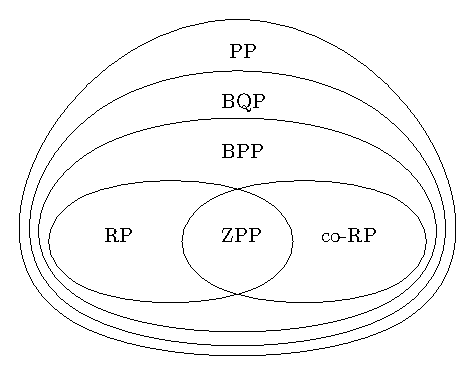
\includegraphics{img/rp-hierarchy.eps}
	\caption{Hierarchie pravděpodobnostních tříd}
\end{figure}

\vt P $\subseteq$ RP, ZPP $\subseteq$ RP

\tv (P ?= BPP) Je otevřený problém, zda P $=$ BPP. Pokud ano, pak P, RP, co-RP a
ZPP jsou si rovny.

\tv (Zero Polynomial Testing) Algoritmus na testování, zda je polynom ve více
proměnných roven nulovému polynomu, je v co-RP, ale  neví se, zda je v P.

\df (Monte Carlo, Las Vegas) Algoritmus, který běží v polynomiálním čase, ale
může vydat špatný výsledek, je {\bf Monte Carlo}. Algoritmus, který běží v
randomizovaném čase, ale vydá správný výsledek vždy, je {\bf Las Vegas}


\end{document}
